\section*{Data and Resources}
\label{sec:data}

\subsection{Data Collections}

In this artcile we investigated methods to estimate Web page understandability, including the effect HTML preprocessing pipelines and heuristics have, and their search effectiveness when employed within retrieval methods. To obtain both topical relevance\footnote{We refer to this simply as relevance in the reminder of the paper, when this does not cause confusion.} and  understandability assessments, we used the data from the CLEF 2015 and 2016 eHealth collections. 

The CLEF 2015 collection contains 50 queries and 1,437 documents that have been assessed relevant by clinical experts and have an assessment for understandability~\cite{clef15}. Documents in this collection are a selected crawl of health Web sites, of which the majority are certified HON Web sites.
The CLEF 2016 collection contains 300 queries and 3,298 relevant documents that also have been assessed with respect to understandability~\cite{clef16}. Documents in this collection belong to the ClueWeb12 B13 corpus, and thus are general English Web pages, not necessarily targeted to health topics, nor of a controlled quality (as are instead HON certified pages). 
Understandability assessments were provided on a 5-point Likert scale for CLEF 2015, and on a $[0,100]$ range for CLEF 2016 (0 indicates highest understandability). 

To support the investigation on methods to automatically estimate the understandability of Web pages, 
%in Section~\ref{sec:which_preprocessing} (evaluation of preprocessing pipelines and heuristics), 
we further considered correlations between multiple human assessors (inter-assessor agreement). For CLEF 2015, we used the publicly available additional assessments made by unpaid medical students and health consumers collected by Palotti et al.~\cite{palotti16b} in a study of how medical expertise affects assessments. For CLEF 2016 we  collected understandability assessments for 100 documents. Three members of our research team, which did not author this paper, were recruited to provide the assessments. The Relevation tool~\cite{koopman14} was used to assist with the assessments, mimicking the settings used in CLEF. \mytodo{should we briefly show these results?}

\subsection{Evaluation Measures}

In the experiments, we used Pearson, Kendall and Spearman correlations to compare the understandability assessments of human assessors with estimations obtained by the considered approaches, under all combinations of pipelines and heuristics. Pearson correlation is used to calculate the strength of the linear relation between two variables, while Kendall and Spearman measure the rank correlations between the variables. We opted to report all three correlation coefficients to allow for a thorough comparison to other work, as they are equally used in the literature. 

For the retrieval experiments in Section~\ref{sec:results}, we used evaluation measures that use both relevance and understandability. The uRBP measure~\cite{zuccon2016understandability} extends rank biased precision (RBP) to scenarios where multiple relevance dimensions are used. The measure is formulated as $uRBP(\rho) = (1 - \rho) \sum_{k=1}^{K} \rho^{k-1} r(d@k) u(d@k)$, where $r(d@k)$ is the gain for retrieving a relevant document at rank $k$ and $u(d@k)$ is the gain for retrieving a document of a certain understandability at rank $k$; $\rho$ is the RBP persistence parameter. This measure was an official evaluation measure used in CLEF (we also set $\rho=0.8$). 

A drawback of uRBP is that relevance and understandability are combined into a unique evaluation score, thus making it difficult to interpret whether improvements are due to more understandable or more topical documents being retrieved. To overcome this, we first separately calculated an RBP value for relevance and another for understandability, and then combined them into a unique effectiveness measure:

\begin{itemize}[leftmargin=*]
	\item $RBP_r@n(\rho)$: uses the relevance assessments for the top $n$ search results (i.e. this is the common RBP). We regarded a document as topically relevant if assessed as somewhat relevant or highly relevant.
	
    \item $RBP_u@n(\rho)$: uses the understandability assessments for the top $n$ search results. We regarded a document as understandable (1) for CLEF 2015 if assessed easy or somewhat easy to understand; (2) for CLEF 2016 if its assessed understandability score was smaller than a threshold $U$ (we used $U = 40$ \footnote{This choice for $U$ was based on the distribution of understandability assessments. This distribution can be found in the online appendix.}).
	
    \item $H_{RBP}@n(\rho) = 2 \times \frac{RBP_r@n \times RBP_u@n}{RBP_r@n + RBP_u@n}$: combines the previous two RBP values into a unique measurement using the harmonic mean (in the same fashion that the $F_1$ measure combines recall and precision).
\end{itemize}

\noindent For all measures we set $n=10$ because shallow pools were used in CLEF along with measures that focused on the top 10 search results (including $RBP_r@10$).

Along with these measures of search effectiveness, we also reported the number of unassessed documents, the RBP residuals,  $RBP_r@10^*$, $RBP_u@10^*$ and $H_{RBP}^*$, i.e. the corresponding measures calculated by ignoring unassessed documents. We did this to minimise pool bias since the pools built in CLEF were of limited size, and the investigated methods retrieved a substantial number of unassessed documents.


\subsection{Preprocessing Pipelines and Heuristics}
\label{sec:pipelines}

As part of our study, we investigated the influence the preprocessing of Web pages has on the estimation of understandability, when this is estimated using the methods in Section~\ref{sec:proxies}. We did so by comparing the combination of a number of preprocessing pipelines, heuristics, and understandability estimation methods with human assessments of Web page understandability. 
Our experiments extended those by Palotti et al.~\cite{palotti15}, who only evaluated surface level readability formulas and did not compare their results against human assessments. 
\mytodo{NEW CONTRIBUTION FOUND...}

To extract the content of a Web page from the HTML source we tested: BeautifulSoup\footnote{\url{https://www.crummy.com/software/BeautifulSoup/}} (\textit{Naive}), which just naively removes HTML tags, Boilerpipe~\cite{kohlschutter10} (\textit{Boi}) and Justext~\cite{jan11} ({Jst}), which eliminates boilerplate text together with HTML tags. 
%Palotti et al.'s data analysis highlighted that the text in HTML tags often missed a correct punctuation mark and thus the text extracted from HTML fields like titles, menus, tables and lists could be interpreted as many short sentences or few very long sentences, depending on whether a period was forced at the end of fields/sentences. We thus implement the same two heuristics devised by them to deal with this: \textit{ForcePeriod (FP)} and \textit{DoNotForcePeriod (DNFP)}. The FP heuristic forces a period at the end of each extracted HTML field; while the DNFP does not. 
Palotti et al.'s data analysis highlighted that the text in HTML fields like titles, menus, tables and lists often missed a correct punctuation mark and thus the text extracted from them could be interpreted as many short sentences or few very long sentences, depending on whether a period was forced at the end of fields/sentences. We thus implemented the same two heuristics devised by Palotti et al. to deal with this: \textit{ForcePeriod (FP)} and \textit{DoNotForcePeriod (DNFP)}. The FP heuristic forces a period at the end of each extracted HTML field, while the DNFP does not. 


\subsection{Additional Resources}

Because of space limitations, in this article we only reported a subset of the results; the remaining results (which show similar trends to those reported here) are made available in an online appendix for completeness: {\url{https://sites.google.com/view/understandabilityontheweb/}. All data and code will be shared on GitHub upon acceptance.
\mytodo{Check what can we integrate from the google site and put here.}
\mytodo{Modify google site page to something that has no journal name.}

%\begin{figure*}[th!]
%   \centering
%   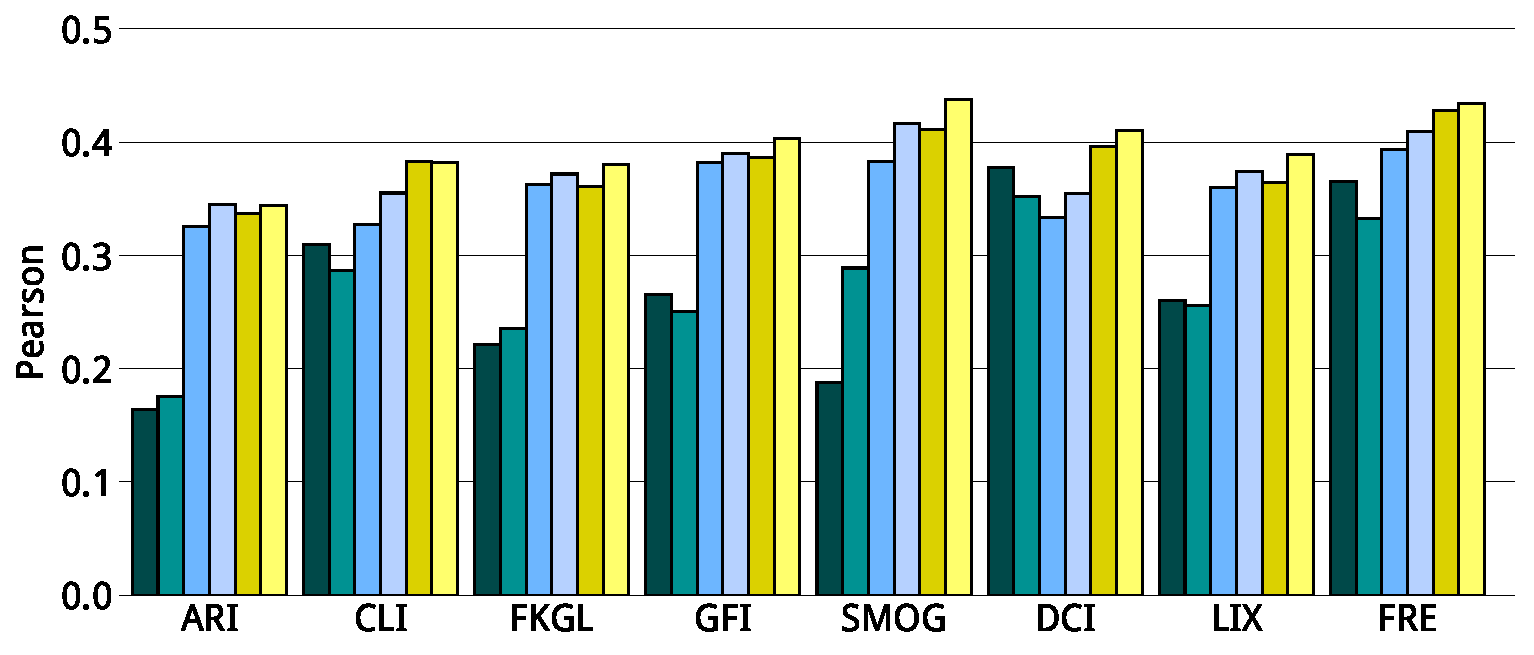
\includegraphics[width=.45\textwidth]{graphics/bar_corr_pearson15_values}
%   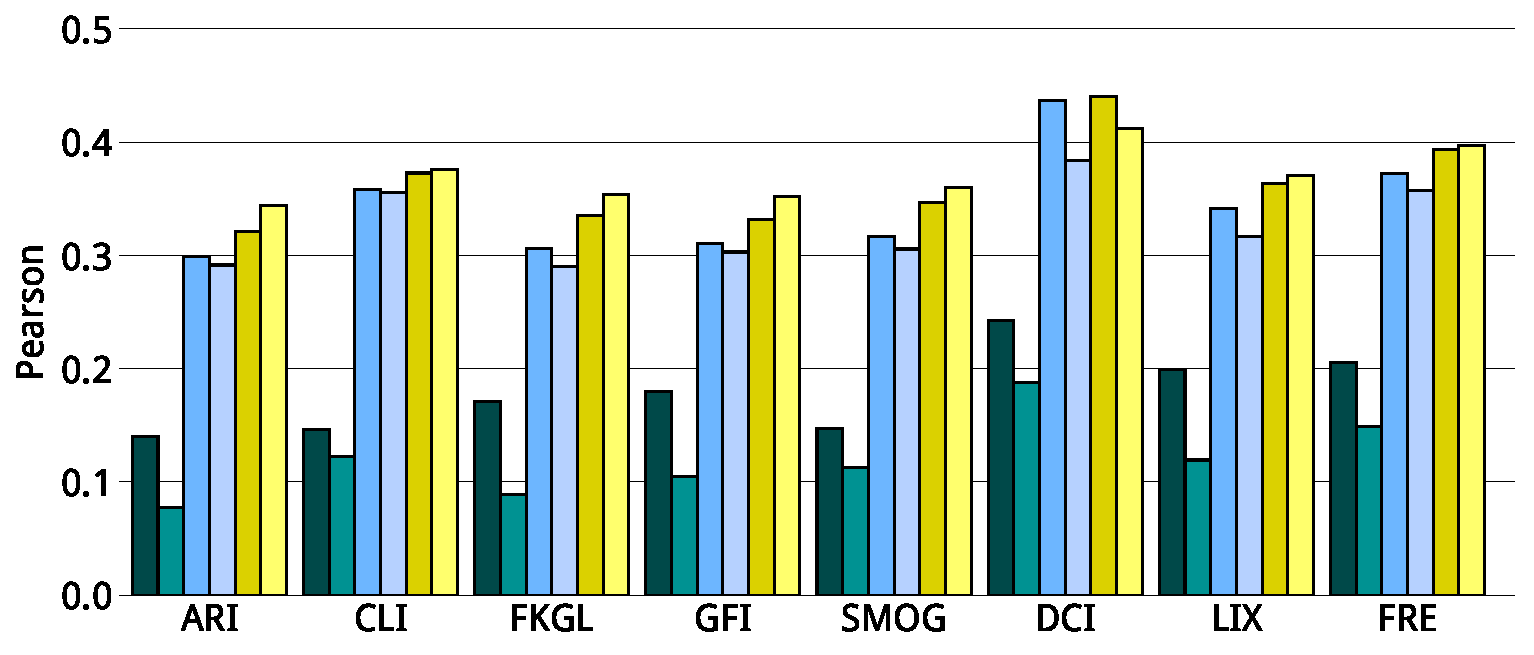
\includegraphics[width=.45\textwidth]{graphics/bar_corr_pearson16_values}
%   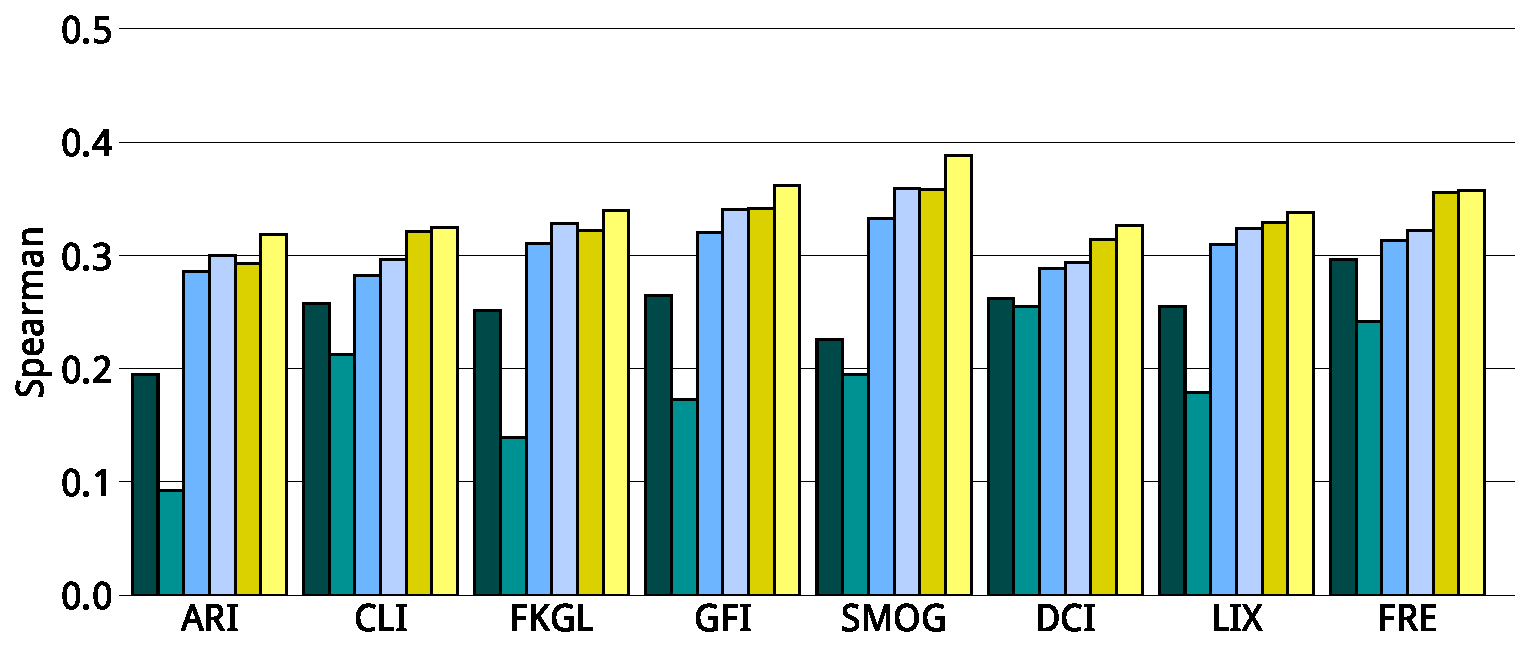
\includegraphics[width=.45\textwidth]{graphics/bar_corr_spearman15_values}
%   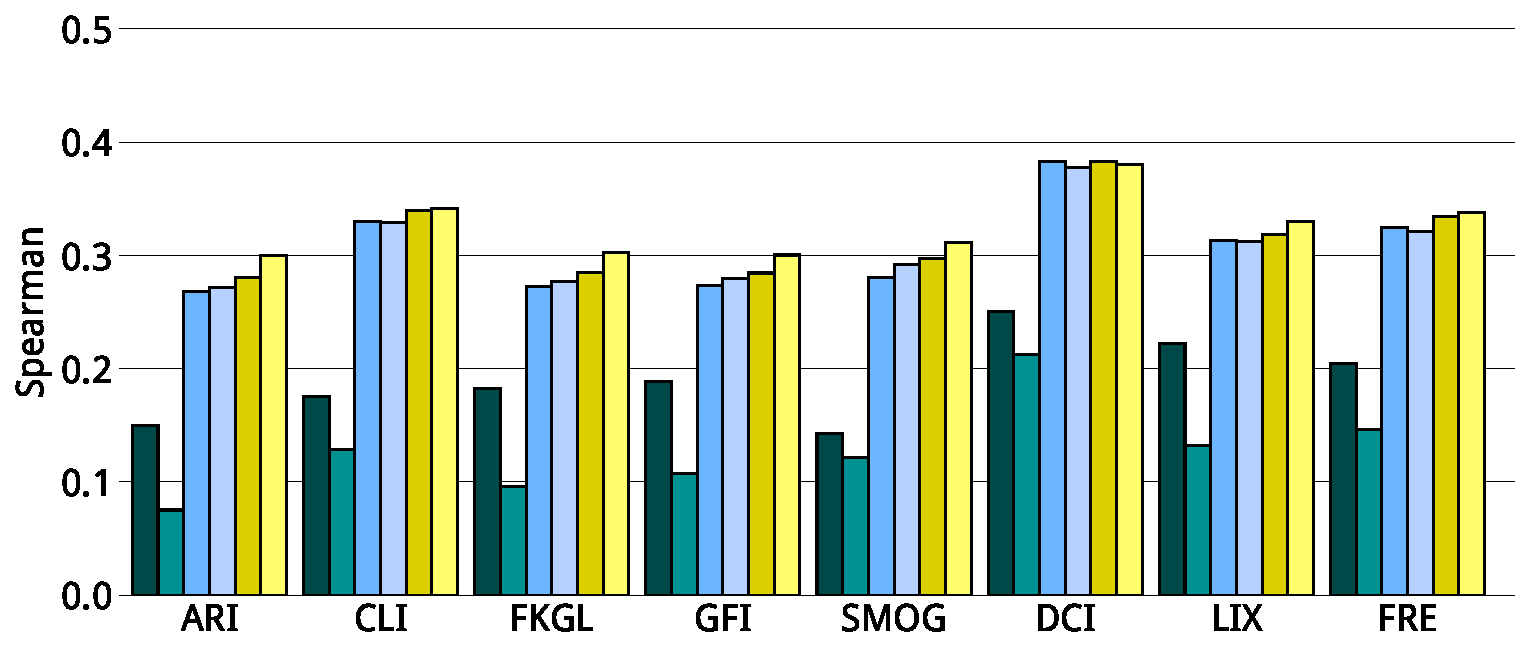
\includegraphics[width=.45\textwidth]{graphics/bar_corr_spearman16_values}
%   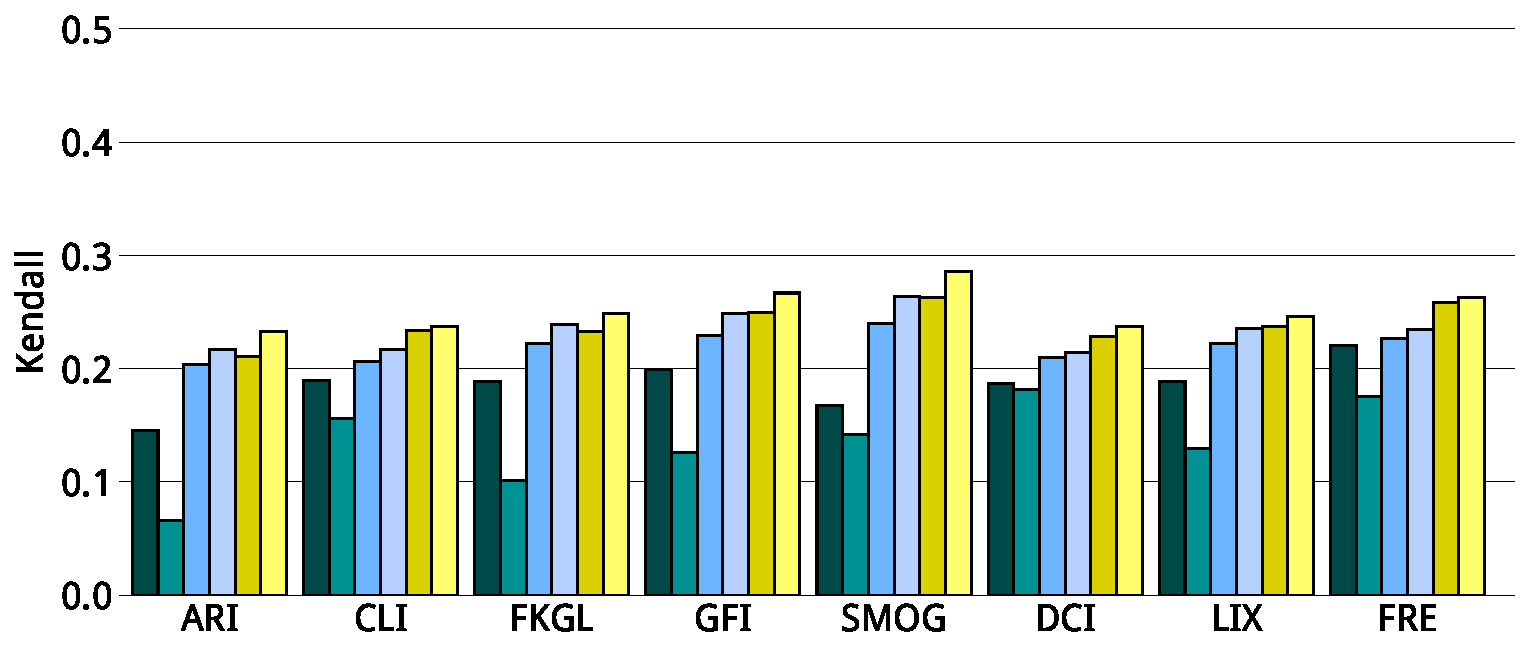
\includegraphics[width=.45\textwidth]{graphics/bar_corr_kendalltau15_values}
%   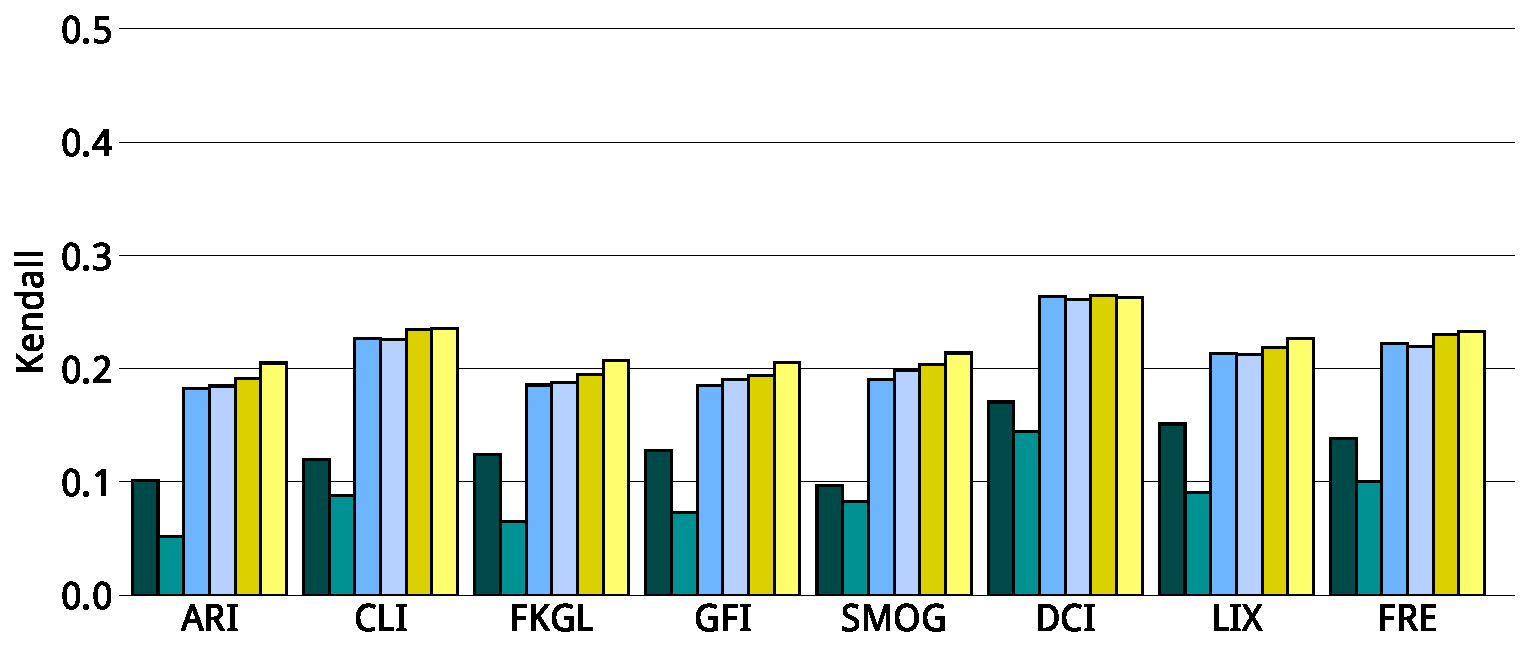
\includegraphics[width=.45\textwidth]{graphics/bar_corr_kendalltau16_values}
%   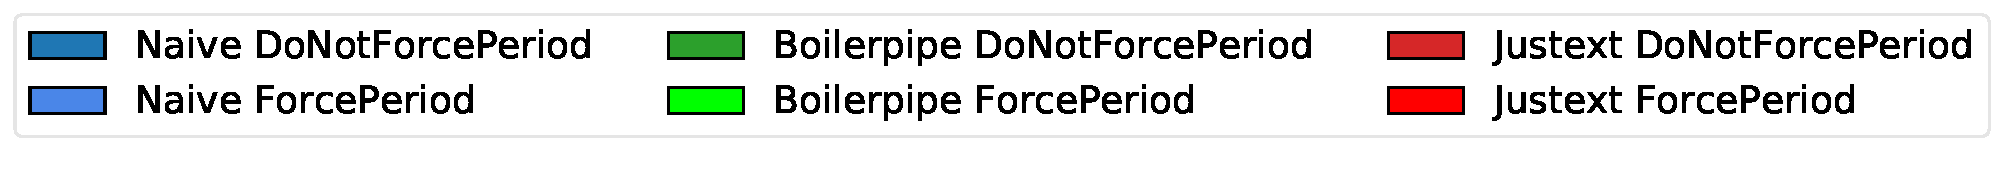
\includegraphics[width=.8\textwidth]{graphics/legend62}
%    \caption{Absolute correlation coefficient of different readability measures and understandability scores. On the left hard side, CLEF eHealth 2015, on the right hand side, CLEF eHealth 2016}
%   \label{fig:bar_corr_clef15}
%\end{figure*}

%\begin{figure*}[th!]
%  \centering
%   \caption{Correlation of different readability measures and the understandability scores collected in CLEF eHealth 2016.}
%  \label{fig:bar_corr_clef16}
%\end{figure*}


